%!TEX program = xelatex
\documentclass[dvipsnames, svgnames,a4paper,11pt]{article}
% ----------------------------------------------------
%   中山大学物理与天文学院本科实验报告模板
%   作者:Huanyu Shi,2019级
%   知乎:https://www.zhihu.com/people/za-ran-zhu-fu-liu-xing
%   Github:https://github.com/Huanyu-Shi/SYSU-SPA-Labreport-Template
%   Last update : 2023.4.10
% ----------------------------------------------------

% ----------------------------------------------------- 
%	加边框的命令
%	参考:https://tex.stackexchange.com/questions/531559/how-to-add-the-page-border-for-first-two-pages-in-latex
\usepackage{tikz}
\usetikzlibrary{calc}
\usepackage{eso-pic}
\AddToShipoutPictureBG{%
\begin{tikzpicture}[overlay,remember picture]
\draw[line width=0.6pt] % 边框粗细
    ($ (current page.north west) + (0.6cm,-0.6cm) $)
    rectangle
    ($ (current page.south east) + (-0.6cm,0.6cm) $); % 边框位置
\end{tikzpicture}}


\usepackage{xcolor}
\definecolor{c1}{HTML}{2752C9} % 目录颜色
\definecolor{c2}{RGB}{190,20,83} % 引用颜色

\usepackage{ctex}
\usepackage[top=28mm,bottom=28mm,left=15mm,right=15mm]{geometry}
\usepackage{hyperref} 
\hypersetup{
	colorlinks,
	linktoc = section, % 超链接位置,选项有section, page, all
	linkcolor = c1, % linkcolor 目录颜色
	citecolor = c1  % citecolor 引用颜色
}
\usepackage{amsmath,enumerate,multirow,float}
\usepackage{tabularx}
\usepackage{tabu}
\usepackage{subfig}
\usepackage{fancyhdr}
\usepackage{graphicx}
\usepackage{wrapfig}  
\usepackage{physics}
\usepackage{appendix}
\usepackage{amsfonts}

%
\usepackage{tcolorbox}
\tcbuselibrary{skins,breakable}
\newtcolorbox{tbox}[2][]{
    colframe=black!70!,
    breakable,
    enhanced,
	boxrule =0.5pt,
    title = {#2},
    fonttitle = \large\kaishu\bfseries,
	drop fuzzy shadow,
    #1
}
\newtcolorbox[auto counter,number within=section]{question}[1][]{
  top=2pt,bottom=2pt,arc=1mm,
  boxrule=0.5pt,
%   frame hidden,
  breakable,
  enhanced, %跨页后不会显示下边框
  coltitle=c1!80!gray,
  colframe=c1,
  colback=c1!3!white,
  drop fuzzy shadow,
  title={思考题~\thetcbcounter:\quad},
  fonttitle=\bfseries,
  attach title to upper,
  #1
}
\newcommand{\setLhead}[1]{%
  \lhead{{\color{gray}\kaishu #1}} % 定义新的命令,设置右边页眉的内容
}
\newcommand{\setRhead}[1]{%
  \rhead{{\color{gray}\kaishu #1}} % 定义新的命令,设置右边页眉的内容
}
% ---------------------------------------------------------------------
%	利用cleveref改变引用格式,\cref是引用命令
\usepackage{cleveref}
\crefformat{figure}{#2{\textcolor{c2}{图 #1}}#3} % 图片的引用格式
\crefformat{equation}{#2{(\textcolor{c2}{#1})}#3} % 公式的引用格式
\crefformat{table}{#2{\textcolor{c2}{表 #1}}#3} % 表格的引用格式


% ---------------------------------------------------------------------
%	页眉页脚设置
\fancypagestyle{plain}{\pagestyle{fancy}}
\pagestyle{fancy}
\setLhead{中山大学物理与天文学院基础物理实验预习报告}
%\lhead{\kaishu 中山大学物理与天文学院物理实验\uppercase\expandafter{\romannumeral3}} % 左边页眉,学院 + 课程
%\rhead{{\color{gray}\kaishu Template 实验报告模板}} % 右边页眉,实验报告标题
\setRhead{实验1\hspace{1pt}冰的熔化热测量}
\cfoot{\thepage} % 页脚,中间添加页码


% ---------------------------------------------------------------------
%	对目录、章节标题的设置
\renewcommand{\contentsname}{\centerline{\huge 目录}}
\usepackage{titlesec}
\usepackage{titletoc}
% \titleformat{章节}[形状]{格式}{标题序号}{序号与标题间距}{标题前命令}[标题后命令]
\titleformat{\section}{\centering\LARGE\songti}{}{1em}{}

% ---------------------------------------------------------------------
%   listing代码环境设置
\usepackage{listings}
\lstloadlanguages{python}
\lstdefinestyle{pythonstyle}{
backgroundcolor=\color{gray!5},
language=python,
frameround=tftt,
frame=shadowbox, 
keepspaces=true,
breaklines,
columns=spaceflexible,                   
basicstyle=\ttfamily\small, % 基本文本设置,字体为teletype,大小为scriptsize
keywordstyle=[1]\color{c1}\bfseries, 
keywordstyle=[2]\color{Red!70!black},   
stringstyle=\color{Purple},       
showstringspaces=false,
commentstyle=\ttfamily\scriptsize\color{green!40!black},%注释文本设置,字体为sf,大小为smaller
tabsize=2,
morekeywords={as},
morekeywords=[2]{np, plt, sp},
numbers=left, % 代码行数
numberstyle=\it\tiny\color{gray}, % 代码行数的数字字体设置
stepnumber=1,
rulesepcolor=\color{gray!30!white}
}




% ---------------------------------------------------------------------
%	其他设置
\def\degree{${}^{\circ}$} % 角度
\graphicspath{{./images/}} % 插入图片的相对路径
\allowdisplaybreaks[4]  %允许公式跨页 % 导入模板的相关设置
\usepackage{lipsum}
\usepackage{indentfirst}
\usepackage{pdfpages}
\usepackage{multirow}
\usepackage{subfig}
\usepackage{graphicx}
\usepackage{float} 
\usepackage{booktabs}
\usepackage{enumerate}
\usepackage{makecell} 
\usepackage{diagbox}
\renewcommand{\d}{\mathrm{d}}
\newcommand{\upcite}[1]{\textsuperscript{\textsuperscript{\cite{#1}}}}


%---------------------------------------------------------------------
%	正文
%---------------------------------------------------------------------
\setRhead{透镜组基本参数的测量}%实验名称
\begin{document}


\begin{table}
	\renewcommand\arraystretch{1.7}
	\begin{tabularx}{\textwidth}{
		|X|X|X|X
		|X|X|X|X|}
	\hline
	\multicolumn{2}{|c|}{预习报告}&\multicolumn{2}{|c|}{实验记录}&\multicolumn{2}{|c|}{分析讨论}&\multicolumn{2}{|c|}{总成绩}\\
	\hline
	 & &  & &  & &  & \\
	\hline
	\end{tabularx}
\end{table}


\begin{table}
	\renewcommand\arraystretch{1.7}
	\begin{tabularx}{\textwidth}{|X|X|X|X|}
	\hline
	专业:& 物理学类 &年级:& 2023级\\
	\hline
	姓名:& 姚昊廷  & 学号:&22322091\\
	\hline
	实验时间:& 2024.12.26& 教师签名:& \\
	\hline
	\end{tabularx}
\end{table}

\begin{center}
	\LARGE 透镜组基本参数的测量
\end{center}

\textbf{【实验报告注意事项】}
\begin{enumerate}
	\item 实验报告由三部分组成:
	\begin{enumerate}
		\item 预习报告:(提前一周)认真研读\underline{\textbf{实验讲义}},弄清实验原理;实验所需的仪器设备、用具及其使用(强烈建议到实验室预习),完成课前预习思考题;了解实验需要测量的物理量,并根据要求提前准备实验记录表格(第一循环实验已由教师提供模板,可以打印)。预习成绩低于10分(共20分)者不能做实验。
	    \item 实验记录:认真、客观记录实验条件、实验过程中的现象以及数据。实验记录请用珠笔或者钢笔书写并签名(\textcolor{red}{\textbf{用铅笔记录的被认为无效}})。\textcolor{red}{\textbf{保持原始记录,包括写错删除部分,如因误记需要修改记录,必须按规范修改。}}(不得输入电脑打印,但可扫描手记后打印扫描件);离开前请实验教师检查记录并签名。
	    \item 分析讨论:处理实验原始数据(学习仪器使用类型的实验除外),对数据的可靠性和合理性进行分析;按规范呈现数据和结果(图、表),包括数据、图表按顺序编号及其引用;分析物理现象(含回答实验思考题,写出问题思考过程,必要时按规范引用数据);最后得出结论。
	\end{enumerate}
	\textbf{实验报告就是将预习报告、实验记录、和数据处理与分析合起来,加上本页封面。}
	\item 每次完成实验后的一周内交\textbf{实验报告}(特殊情况不能超过两周)。
	\item 除实验记录外,实验报告其他部分建议双面打印。
\end{enumerate}

\textbf{【实验安全与实验室注意事项】}\\
\begin{enumerate}
    \item 实验中需带手套,尽量避免用手直接接触镜片的光学面。若不小心触摸了光学表面,需尽快用镜头纸或擦镜布擦拭干净。
    \item 安装镜片时需在光学平台上尽量靠近台面的高度操作,以免失手跌落摔碎镜片。
    \item 实验平台配件所用固定螺钉需拧紧,以免镜架晃动;但不可过紧,以免损坏。
    \item 实验前需按仪器清单检查光学元件是否齐全,实验结束后按照顺序放回元件盒。
\end{enumerate}

\clearpage
\tableofcontents
\clearpage

\setcounter{section}{0}
\section{透镜组基本参数的测量\ \textbf{预习报告}}
	
\subsection{实验目的}
\begin{enumerate}
    \item 熟悉光具座及其附件的使用。
	\item 了解透镜组基点的概念。
	\item 掌握利用节点架进行透镜组基点的测量方法及其原理 。
\end{enumerate}
\subsection{仪器用具}
\begin{table}[htbp]
	\centering
	\renewcommand\arraystretch{1.6}
	% \setlength{\tabcolsep}{10mm}
	\begin{tabular}{p{0.05\textwidth}|p{0.20\textwidth}|p{0.05\textwidth}|p{0.5\textwidth}}
	\hline
	编号& 仪器用具名称 & 数量 &  主要参数(型号,测量范围,测量精度等) \\
	\hline
	1&白光光源&1&GY-6 型,亮度可调,即溴钨灯\\
	\hline
	2&毫米尺&1&30mm, 精度1mm\\
	\hline
	3&调节架&1&---\\
	\hline
    4&透镜L$_0$&1&F=150mm\\
	\hline
    5&透镜架&1&---\\
	\hline
    6&节点架&1&SZ-28\\
	\hline
    7&凸透镜组&1&F=190mm, f=300mm\\
	\hline
    8&测微目镜&1&CW-1型,6mm,精度0.01mm\\
	\hline
    9&测微目镜架&1&SZ-36\\
	\hline
    10-14&平移底座&5&---\\
	\hline
\end{tabular}
\end{table}


\subsection{原理概述和实验前思考题}
\begin{question}
    什么是透镜组的基本参数(基点)?
    \tcblower
    两个以上薄透镜或者厚透镜组成的共轴球面系统称为透镜组,对称轴称为透镜组的光轴.
    对透镜组来说,单个薄透镜的成像规律己不能简单地推广应用,透镜组己无法像薄透镜那样
    定义光心,故不能简单地将物距、像距等参量定义为物、像到光心的距离.为更方便地描述
    系统在成像上的规律,对系统定义了几个特殊的位置,只要能确定这些特殊的位置,就不需
    要追究光线在透镜组内具体的传播过程,便可用公式法(高斯公式或牛顿公式)或作图法求解
    系统成像的情况.这些特殊位置就是系统的焦点和焦平面、主点和主平面、节点和节平面,
    它们统称为系统的基点和基平面。
\end{question}

\begin{question}
    本实验的误差主要来源,如何减小误差?
    \tcblower
    读数误差,由于透镜底座上未标出刻度,故,读出透镜位置时有较大误差。
\end{question}

\clearpage
\setLhead{中山大学物理与天文学院基础物理实验记录}
\begin{table}
	\renewcommand\arraystretch{1.7}
	\centering
	\begin{tabularx}{\textwidth}{|X|X|X|X|}
	\hline
	专业:& 物理学类 &年级:& 2023级 \\
	\hline
	姓名: &姚昊廷& 学号:&22322091  \\
	\hline
	室温:&$22^\circ$C&实验地点:&A508  14\\
	\hline
	学生签名:& & 评分: &\\
	\hline
	实验时间:& 2024.12.26& 教师签名:&\\
	\hline
	\end{tabularx}
\end{table}
\section{透镜组基本参数的测量\ \textbf{实验记录}}
\subsection{实验内容、步骤、结果}
\subsubsection{透镜组节点和焦距的测定}
\begin{enumerate}
	\item 先借助平面镜,用“自准法”调节毫米尺与准直物镜L0的距离,使毫米尺位于L0的物方焦平面上,则通过L0的光束为平行光
	\item 加入透镜组(L1+L2)和白屏或测微目镜,调共轴,找到节点,记录白屏的位置a, 节点架转轴中心的位置b, 以及透镜组中心位置与节点架转轴中心的偏移量d。
沿节点架导轨移动透镜组并保持L1和L2的距离为6cm不变,再次调节找到节点并测量记录。
\begin{table}[H]
	\centering
	\caption{透镜组节点和焦距的测定}
	\begin{tabular}{c|c|c|c}
		\hline
		\diagbox{测量次序}{测量量} &  a/cm & b/cm & d/cm \\
		\hline
		1&79.62&66.82&-0.50\\
		\hline
		2&83.42&70.21&-0.50\\
		\hline
		3&81.28&68.48&-0.50\\
		\hline
		4&84.42&71.28&-0.50\\
		\hline
		5&85.51&71.91&-0.50\\
		\hline
		6&85.24&72.33&-0.50\\
		\hline
		7&86.12&72.80&-0.50\\
		\hline
	\end{tabular}
\end{table}
等比例作图记录此时白屏,透镜组,透镜组中心位置和节点架转轴中心的相对位置(这里需标注L1, L2对应的焦距值,尤其需要记录透镜组中心位置在节点架转轴中心位置的左侧还是右侧)。
\begin{figure}[H]
	\begin{tikzpicture}[scale=0.8]
		\coordinate (a) at (19.62,0);
        \coordinate (b) at (6.82,0);
        \coordinate (o) at (6.32,0);
        \draw[<->] (3.32,3) --(3.32,-3)node[below]{$f_{L_1}$=300mm};
		\draw[<->] (9.32,3) --(9.32,-3)node[below]{$f_{L_2}$=190mm};
		\draw (19.62,-3) --(19.62,3)node[below]{白屏};
		\draw[loosely dashed] (0,0) --(20,0);
		\filldraw (b) circle (.1)node[below]{节点架转轴中心};
		\filldraw (o) circle (.1)node[above]{透镜组中心};
		\draw (16,-3) --(17,-3)node[below]{1cm};
	\end{tikzpicture}
\end{figure}
\item 将节点架绕z轴转到180度,重复步骤2),测得另一组数据
\begin{table}[H]
	\centering
	\caption{透镜组节点和焦距的测定}
	\begin{tabular}{c|c|c|c}
		\hline
		\diagbox{测量次序}{测量量} & a/cm & b/cm & d/cm \\
		\hline
		1&82.56&70.42&0.30\\
		\hline
		2&83.79&71.21&0.30\\
		\hline
		3&85.05&72.39&0.30\\
		\hline
		4&85.89&73.22&0.30\\
		\hline
		5&87.18&74.68&0.30\\
		\hline
		6&87.91&75.20&0.30\\
		\hline
		7&89.23&76.15&0.30\\
		\hline
	\end{tabular}
\end{table}
等比例作图记录此时白屏,透镜组,透镜组中心位置和节点架转轴中心的相对位置(这里需标注L1, L2对应的焦距值,尤其需要记录透镜组中心位置在节点架转轴中心位置的左侧还是右侧)。
\begin{figure}[H]
	\begin{tikzpicture}[scale=0.8]
		\coordinate (a) at (5.42,0);
        \coordinate (b) at (17.56,0);
        \coordinate (o) at (5.72,0);
        \draw[<->] (2.72,3) --(2.72,-3)node[below]{$f_{L_1}$=190mm};
		\draw[<->] (8.72,3) --(8.72,-3)node[below]{$f_{L_2}$=300mm};
		\draw (17.56,-3) --(17.56,3)node[below]{白屏};
		\draw[loosely dashed] (0,0) --(20,0);
		\filldraw (a) circle (.1)node[below]{节点架转轴中心};
		\filldraw (o) circle (.1)node[above]{透镜组中心};
		\draw (16,-3) --(17,-3)node[below]{1cm};
	\end{tikzpicture}
\end{figure}
\end{enumerate}
\subsubsection{实验过程遇到问题记录}
实验1开始可使得毫米尺像无横向移动,旋转80度后出现轻微横向移动,实验结果可能有误差。
\clearpage
\setLhead{中山大学物理与天文学院基础物理实验分析与讨论}
\begin{table}
	\renewcommand\arraystretch{1.7}
	\begin{tabularx}{\textwidth}{|X|X|X|X|}
	\hline
	专业:& 物理学 &年级:& 2023级\\
	\hline
	姓名: &姚昊廷& 学号:&22322091 \\
	\hline
    日期:&2024.12.26 & 评分: &\\
	\hline
	\end{tabularx}
\end{table}

\section{透镜组基本参数的测量\ \textbf{分析与讨论}}
\subsection{分析与讨论}
一、根据测得的实验数据,给出透镜组焦距值和误差(分析);\\
理论计算焦距值:
\begin{align*}
	f=\frac{1}{\frac{1}{f_1}+\frac{1}{f_2}+\frac{d}{f_1f_2}}=10.36\text{cm}
\end{align*}
实验1:\begin{align*}
	f_i&=|a_i-b_i|\\
	\overline{f}&=\frac{1}{7}\sum_{i=1}^{7}f_i=13.11\text{cm}
	\frac{\overline{f}-f}{f}&=12.7\%
\end{align*}
实验1:\begin{align*}
	f_i&=|a_i-b_i|\\
	\overline{f}&=\frac{1}{7}\sum_{i=1}^{7}f_i=12.62\text{cm}
	\frac{\overline{f}-f}{f}&=8.5\%
\end{align*}
误差来源:\begin{enumerate}
	\item 读数误差
	\item 自准法调节平行光条件未完全调节成功
\end{enumerate}\par
二、等比例画出被测透镜组各种基点(包括物方和像方的焦点,节点,主点)的相对位置(不需要做光路图,但是特别需要标注所做图中透镜L1,
 L2所对应的焦距,透镜组节点距离透镜组中心的相对距离);\\
 \begin{figure}[H]
	\begin{tikzpicture}[font=\small,scale=0.5]
		\coordinate (a) at (14.7,0);
        \coordinate (b) at (15.5,0);
        \coordinate (o) at (15,0);
        \draw[<->] (18,3) --(18,-3)node[below]{$f_{L_1}$=190mm};
		\draw[<->] (12,3) --(12,-3)node[below]{$f_{L_2}$=300mm};
		\draw[loosely dashed] (0,0) --(30,0);
		\filldraw (a) circle (.1);
		\filldraw (o) circle (.1)node[above]{主点};
		\filldraw (b) circle (.1);
		\draw (b) --(15.5,1)node[above]{b(d=0.5cm)};
		\draw (a) --(14.7,-1)node[below]{a(d=0.3cm)};
		\filldraw (28.11,0) circle (.1)node[above]{物方焦点};
		\filldraw (2.38,0) circle (.1)node[above]{像方焦点};
		\draw (16,-5) --(17,-5)node[below]{1cm};
		\node at(22,-4) {a:像方节点};
		\node at(22,-5) {b:物方节点};
	\end{tikzpicture}
\end{figure}\par
三、根据结果分析像方(物方)节点的位置与透镜组连线中心位置是否重合 ?\\
不重合,有一定偏移量d,从测量结果分析可知,此偏移量约为0.4cm不可被忽视。透镜组中心并未落在节点转轴中心。
\subsection{实验后思考题}
\begin{question}
	透镜组基本参数测量,节点架绕Z轴做角度不大的转动时,毫米尺像无横向移动,此时像方节点N’在节点架转轴上,为什么? 请解释其背后的物理原理(建议画出光路图说明)。
	\tcblower
	\begin{figure}[H]
		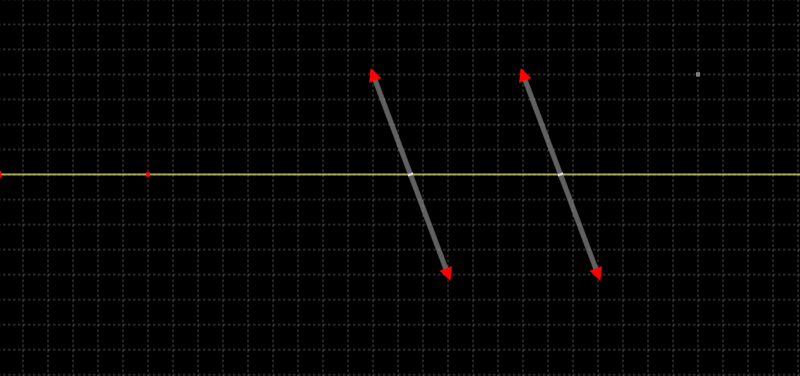
\includegraphics[width=\textwidth]{透镜组光路图.png}
	\end{figure}
	因透镜物方和像方折射率相同有节点和主点位置重合,而主点对像的横向放大率为1。此时节点架的转轴是光线旋转的中心,这个位置是光线会聚的点。
	任何旋转都不会导致像的横向移动。
\end{question}

\begin{question}
	请给出透镜组节点和焦点(距)与其中两个透镜焦距及其间距的关系(作图并用公式说明)。
	\tcblower
	公式:$\frac{1}{f}=\frac{1}{f_1}+\frac{1}{f_2}+\frac{d}{f_1f_2}$\\
	由公式知两透镜间距越大透镜组节点和焦点距越小;
	两个透镜焦距若变大,透镜组节点和焦点距也就越大。
	\begin{figure}[H]
		\centering
		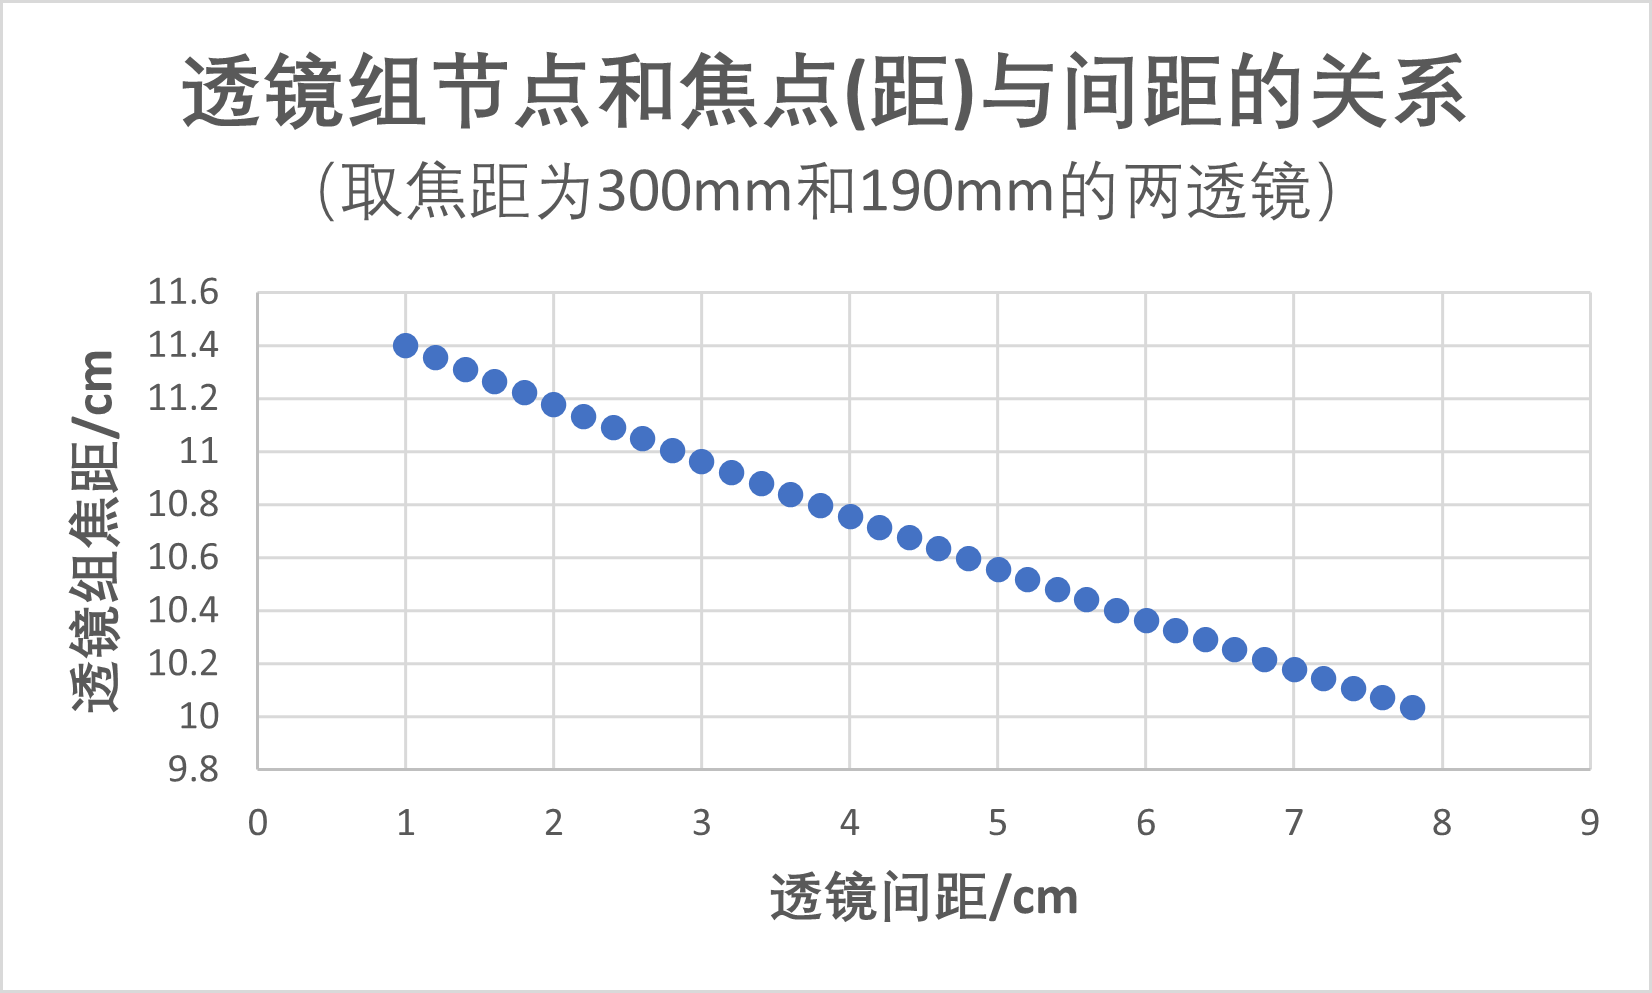
\includegraphics[width=\textwidth]{透镜组1.png}
	\end{figure}
	\begin{figure}[H]
		\centering
		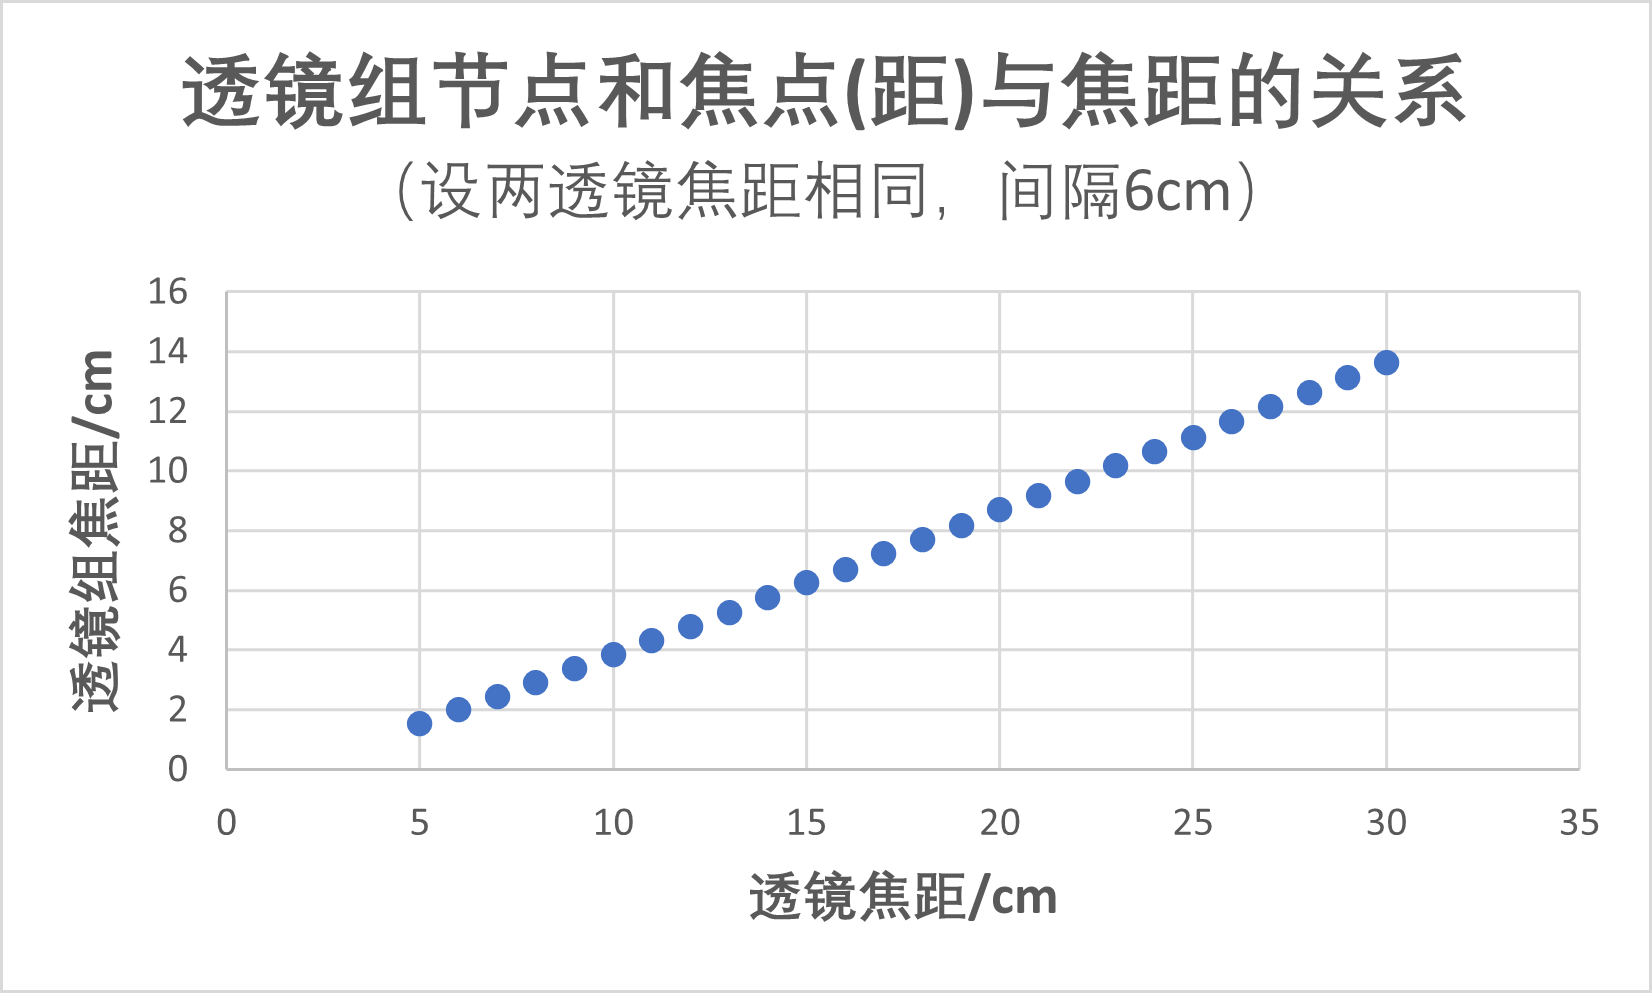
\includegraphics[width=\textwidth]{透镜组2.png}
	\end{figure}
\end{question}
\clearpage
% ---------------------------------------------------------------------
%   参考文献
%   注:使用参考文献时应按照xelatex->bibtex->xelatex->xelatex顺序进行编译
%\phantomsection
%\addcontentsline{toc}{section}{参考文献}
%\bibliographystyle{unsrt}
%\bibliography{myref}
%\begin{thebibliography}{9}
%	\bibitem{ref1} 沈雨欣,翁存程,蒋丽钦.双棱镜干涉法准确测量钠光波长[J].大学物理实验,2023,36(03):40-43.DOI:10.14139/j.cnki.cn22-1228.2023.03.008.
%	\bibitem{ref2} 牟泉润,孙丽媛,杜月棋,等.基于干涉原理的光波长测量装置设计[J].大学物理实验,2021,34(06):80-83+89.DOI:10.14139/j.cnki.cn22-1228.2021.06.018.
%	\bibitem{ref3} 王仁洲,杨涛.一种用激光干涉测量光波波长的新方法[J].大学物理实验,2014,27(06):41-43.DOI:10.14139/j.cnki.cn22-1228.2014.06.014.
%\end{thebibliography}


%\clearpage
\appendix
\appendixpage
\addappheadtotoc
%\subsection*{相图代码}
%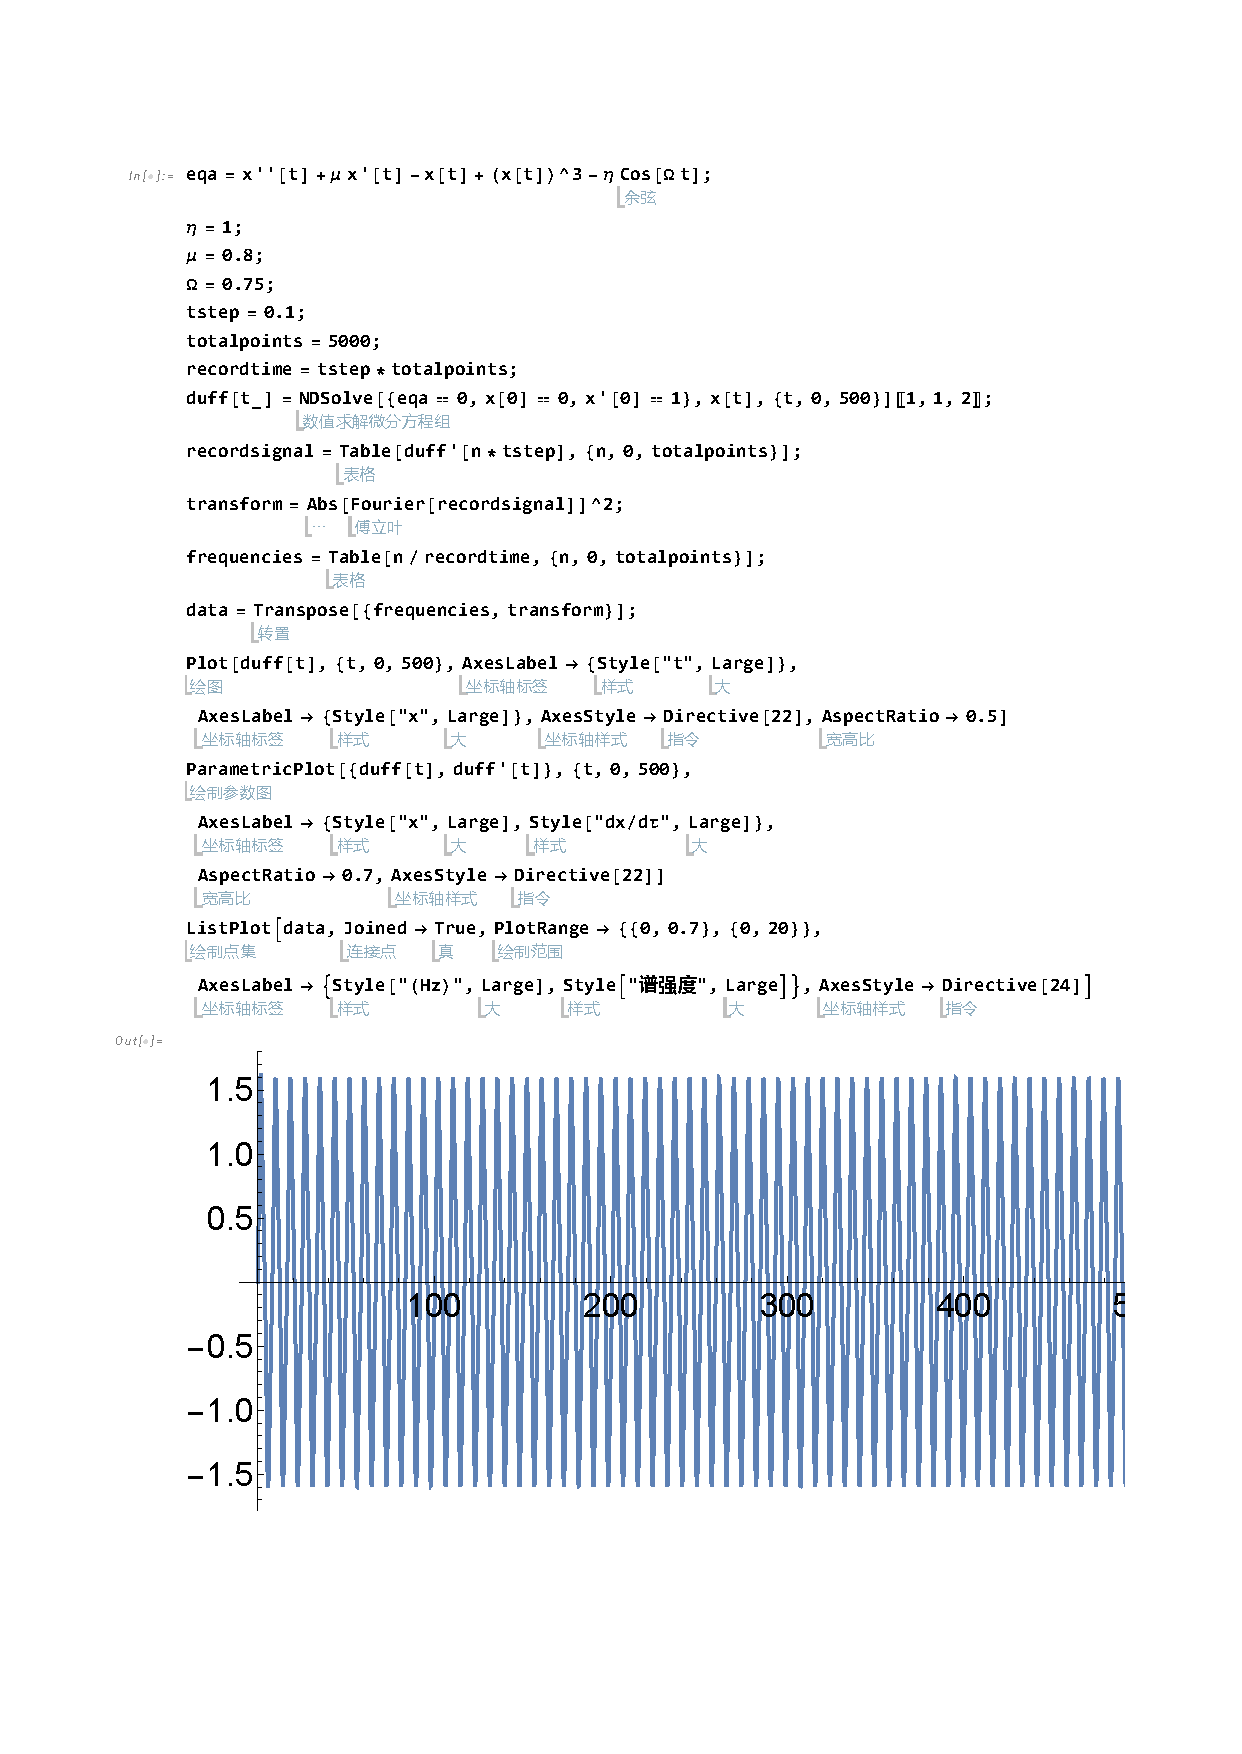
\includepdf[pages=-]{chaos.pdf}
\subsection*{原件}
%\includepdf[pages=-]{原件.pdf}
\begin{figure}[H]
	\centering
	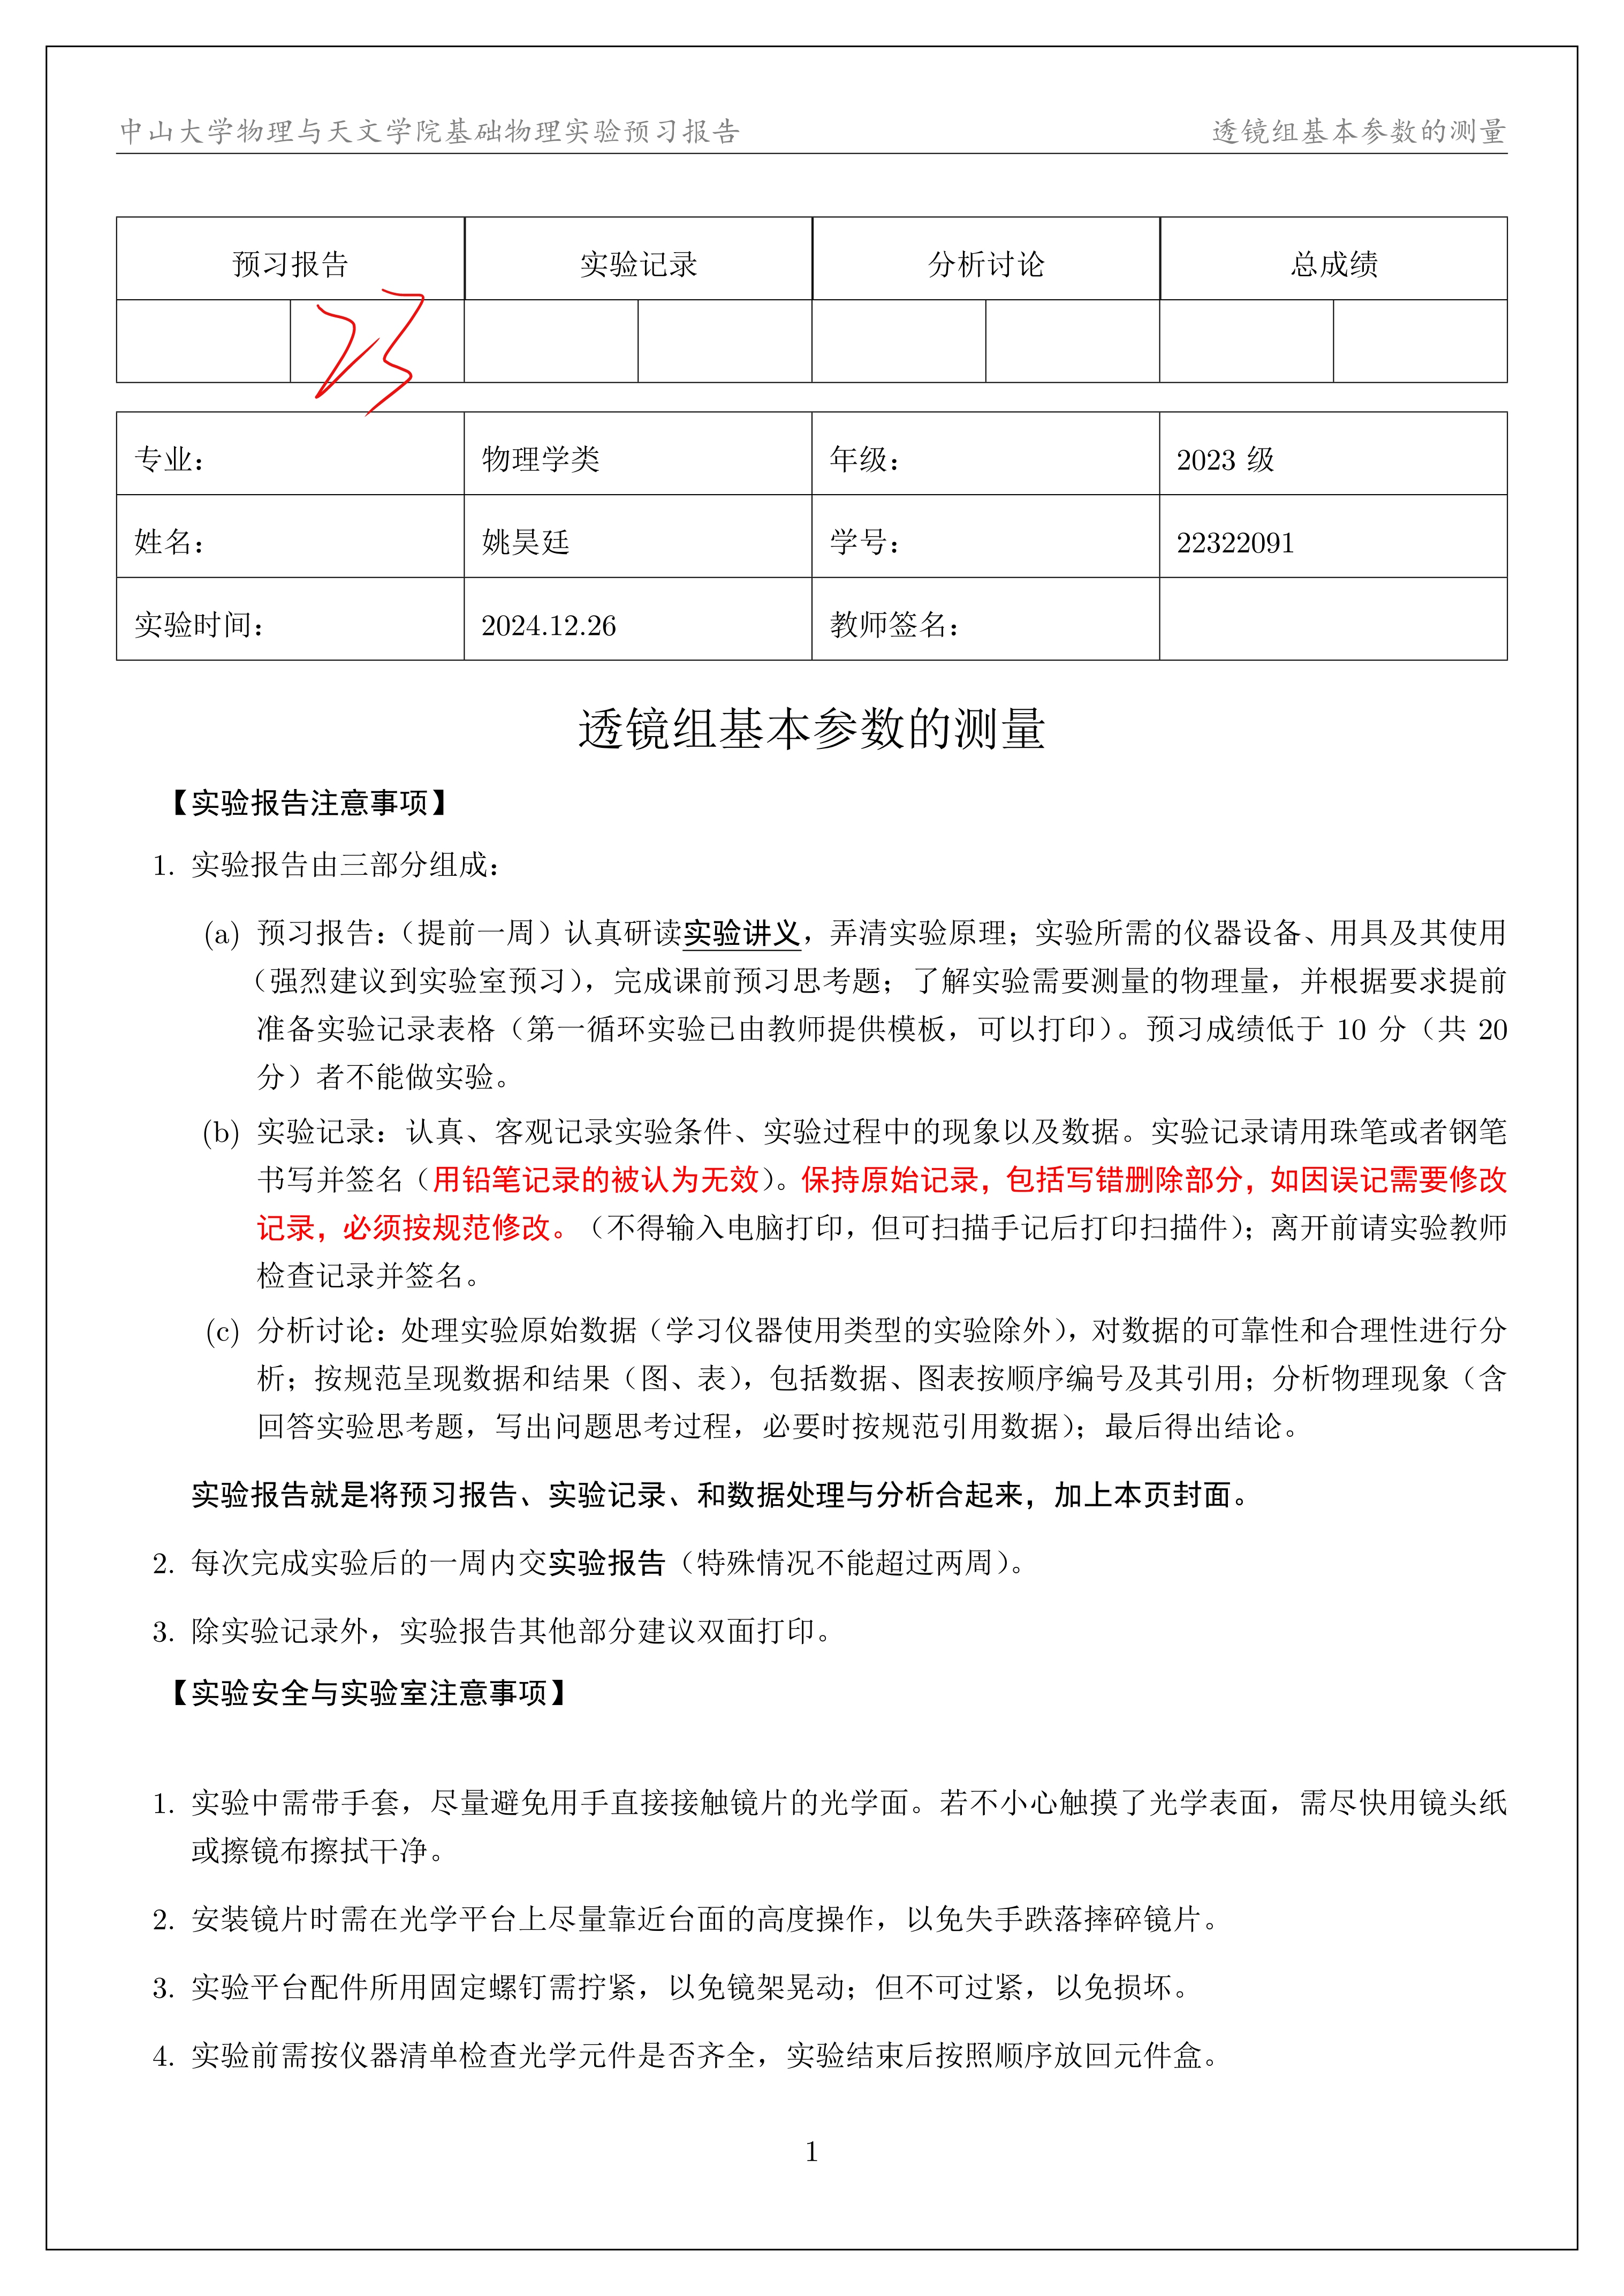
\includegraphics[width=\textwidth]{透镜组原件1.jpg}
	
\end{figure}
\begin{figure}[H]
	\centering
	\includegraphics[width=\textwidth]{透镜组原件2.jpg}
	
\end{figure}

%\begin{figure}[H]
%	\centering
%	\includegraphics[width=0.4\textwidth]{单缝原件1.jpg}
%	\includegraphics[width=0.4\textwidth]{单缝原件2.jpg}
%	\includegraphics[width=0.4\textwidth]{单缝原件3.jpg}
%	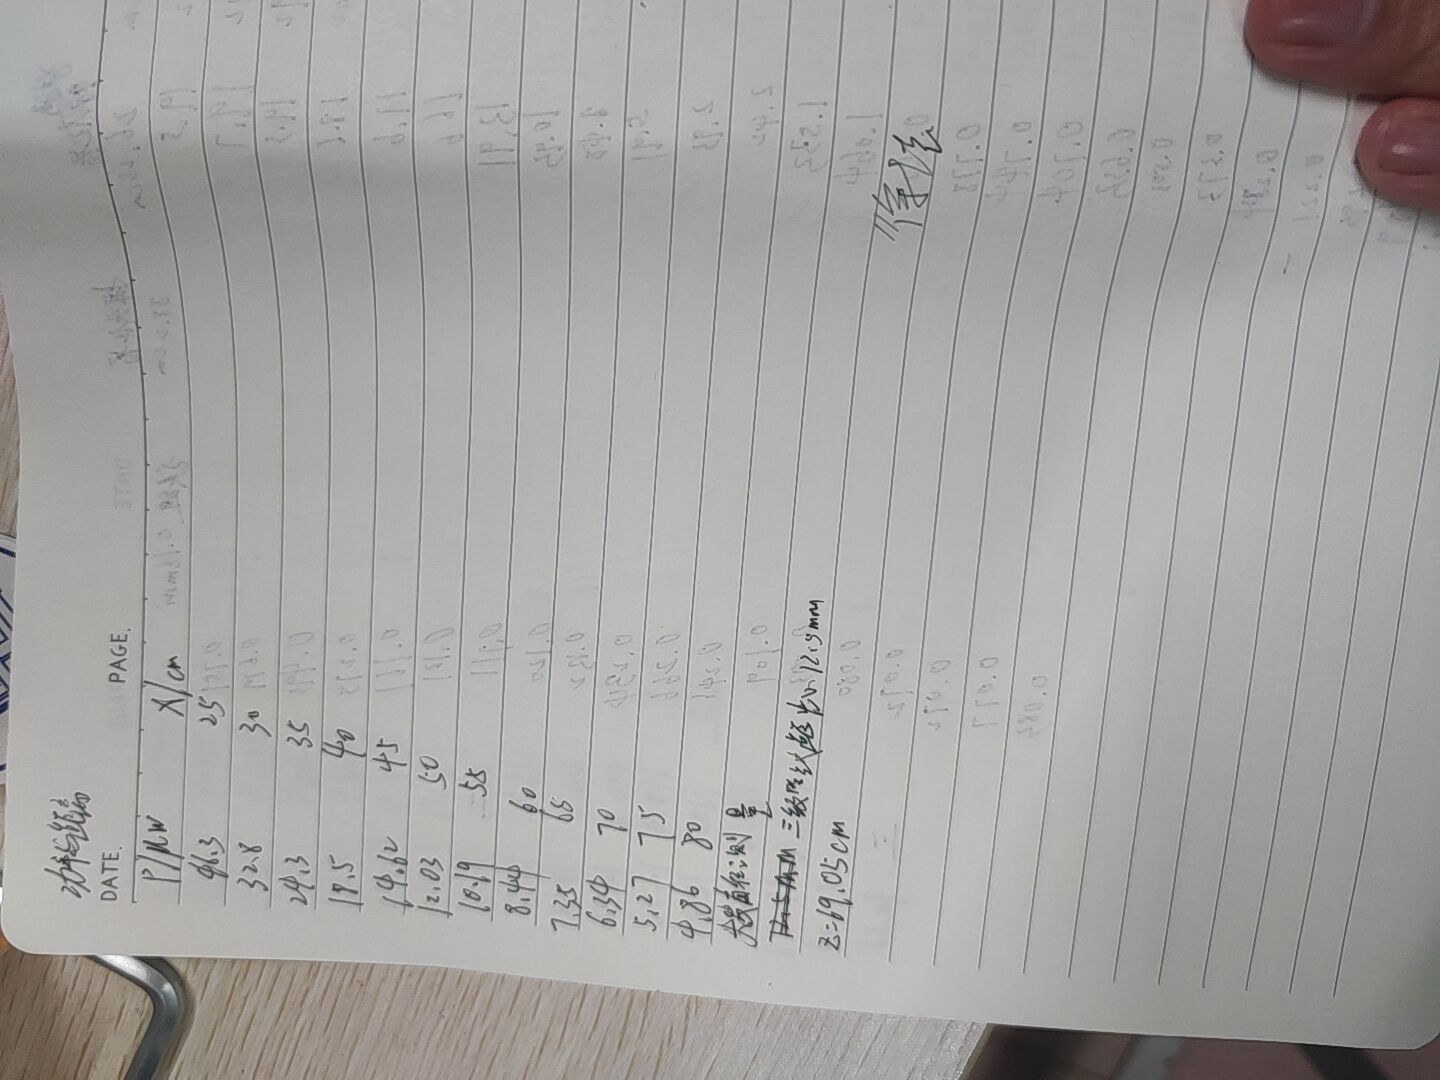
\includegraphics[width=0.4\textwidth]{单缝原件4.jpg}
%\end{figure}
\subsection*{桌面}
\begin{figure}[H]
	\includegraphics[width=0.95\textwidth]{透镜组桌面.jpg}
\end{figure}
\end{document}
%